%! Author = eliainnocenti
%! Date = 16/02/24

% Preamble
\documentclass[11pt]{article}

% Packages % TODO - check
\usepackage{amsmath}
\usepackage{graphicx}
\usepackage{float}
\usepackage{listings}
\usepackage[font=small]{caption}
\usepackage{comment}
\usepackage[linesnumbered,vlined]{algorithm2e}
\usepackage{hhline}
\usepackage{geometry}
\usepackage{tabularx}
\usepackage{hyperref}
\usepackage{xcolor}
\usepackage{tcolorbox}

% Images path
\graphicspath{
        {./resources/images/}
        {../diagrams/}
        {../mockups/}
        {../snippets/}
        {../structure/}
        {../templates/}
}

% Layout settings % TODO - check
\renewcommand{\contentsname}{Index}
\renewcommand{\figurename}{Figure}
\renewcommand{\tablename}{Table}
\SetAlgoCaptionSeparator{}
\geometry{
    bottom=2.8cm
}

% Style % TODO - check
\lstdefinestyle{mystyle}{
    basicstyle=\ttfamily\footnotesize,
    breakatwhitespace=false,
    breaklines=true,
    captionpos=b,
    keepspaces=true,
    numbers=left,
    numbersep=5pt,
    showspaces=false,
    showstringspaces=false,
    showtabs=false,
    tabsize=2
}
\lstset{style=mystyle}

% Document intestation
\title{RendezVous \\
\vspace{0.5em}
\large Software per la creazione e partecipazione di eventi} % FIXME - i don't like it
\author{Elia Innocenti}
\date{Marzo - Aprile 2024}

% Document
\begin{document}

    % FIRST PAGE

    \maketitle

    \vspace{1em}

    \begin{figure}[h]
        \begin{minipage}{\textwidth}
            \centering
            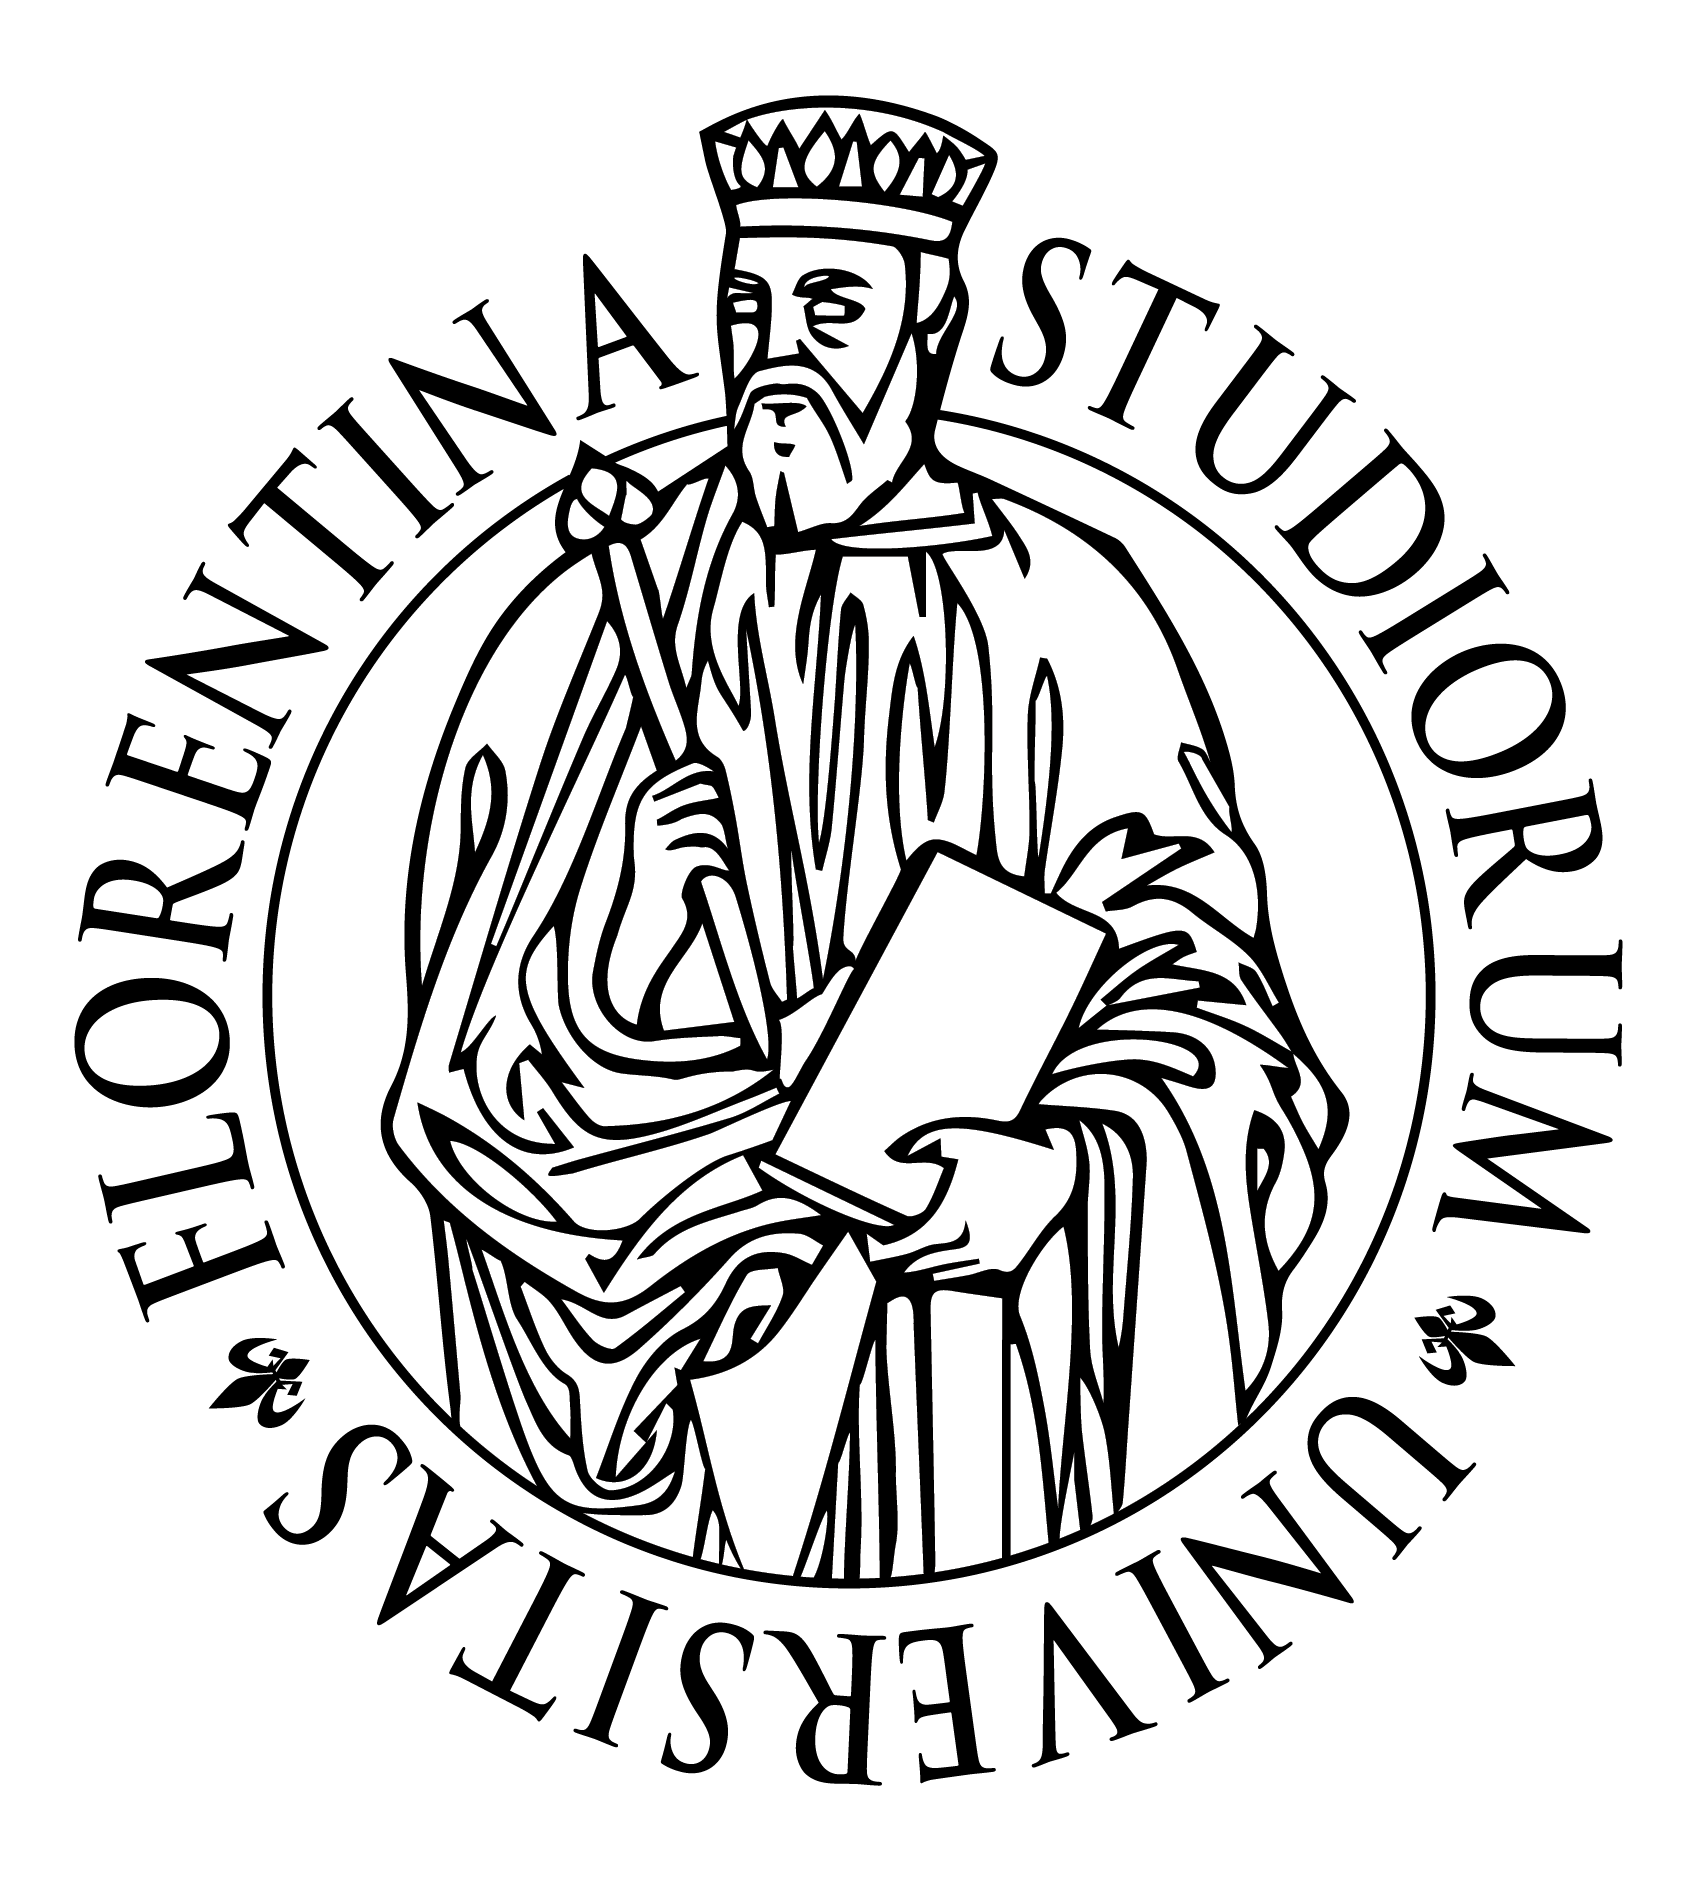
\includegraphics[width=3cm]{unifi-logo}
        \end{minipage}
        \label{fig:uni-logo}
    \end{figure}

    % FIXME - i don't like it
    %\begin{figure}[b]
    %    \begin{minipage}{\textwidth}
    %        \centering
    %        \href{https://github.com/eliainnocenti/RendezVous}{
    %            \hspace{.3em}
    %            \raisebox{0\height}{
\includegraphics[width=1.2cm]{github-logo}}
    %            %\hspace{.3em}
    %            \Large{}
    %        }
    %    \end{minipage}
    %    \label{fig:github-logo}
    %\end{figure}

    % INDEX

    \newpage

    \tableofcontents

    % CONTENT

    \newpage

    \section{Introduzione} \label{sec:introduzione}

        Elaborato per il superamento dell'esame di Ingegneria del Software, appartenente al modulo Basi di Dati / Ingegneria del Software del corso di Laurea Triennale in Ingegneria Informatica dell'Università degli Studi di Firenze.

        \subsection{Obiettivo e descrizione del progetto} \label{subsec:obiettivi-e-descrizione-del-progetto}

            Con questo progetto si sviluppa un programma che permette la creazione di eventi e la partecipazione agli stessi.
            Comprende un sistema di più utenti che possono creare eventi, partecipare a quelli creati da altri utenti pagando la rispettiva quota e gestire il proprio profilo.
            Gli utenti possono effettuare il pagamento tramite carta di credito o PayPal.
            È stato implementato un sistema di amministrazione attraverso un utente admin che permette di gestire gli utenti, gli eventi e le partecipazioni.
            Inoltre per la gestione e il salvataggio dei dati è stato creato e connesso un database.

        \subsection{Struttura e pratiche utilizzate} \label{subsec:struttura-e-pratiche-utilizzate}

            Il software è stato sviluppato in Java, mentre per la gestione del database è stato utilizzato PostgreSQL e
            la libreria JDBC (Java DataBase Connectivity). \\ % TODO: rewrite

            % TODO: introduce the fact that there's also an interface
            Per mantenere una separazione delle responsabilità, la struttura del progetto è stata divisa in tre parti principali: Domain Model, Business Logic e ORM.
            Questi tre packages si occupano in modo distinto de la rappresentazione dei dati, la logica di business e l'accesso ai dati (Figura \ldots): % TODO: insert the name of the figure below (ref)
            \begin{itemize}
                \item \textbf{Domain Model}: contiene le classi che rappresentano le entità del sistema.
                \item \textbf{Business Logic}: contiene le classi che implementano la logica di business del sistema.
                \item \textbf{ORM}: contiene le classi che implementano l'Object-Relational Mapping. In questo modo è possibile rendere
                                    i dati persistenti e recuperarli dal database.
            \end{itemize}

            % TODO: rewrite (copied)
            I diagrammi delle classi e dei casi d’uso seguono lo standard UML (Unified Modeling Language) e sono stati realizzati con il software StarUML. Infine, il testing è stato effettuato tramite i framework JUnit.

            % TODO: insert the dependencies diagram figure
            \begin{figure}[H]
                \centering
                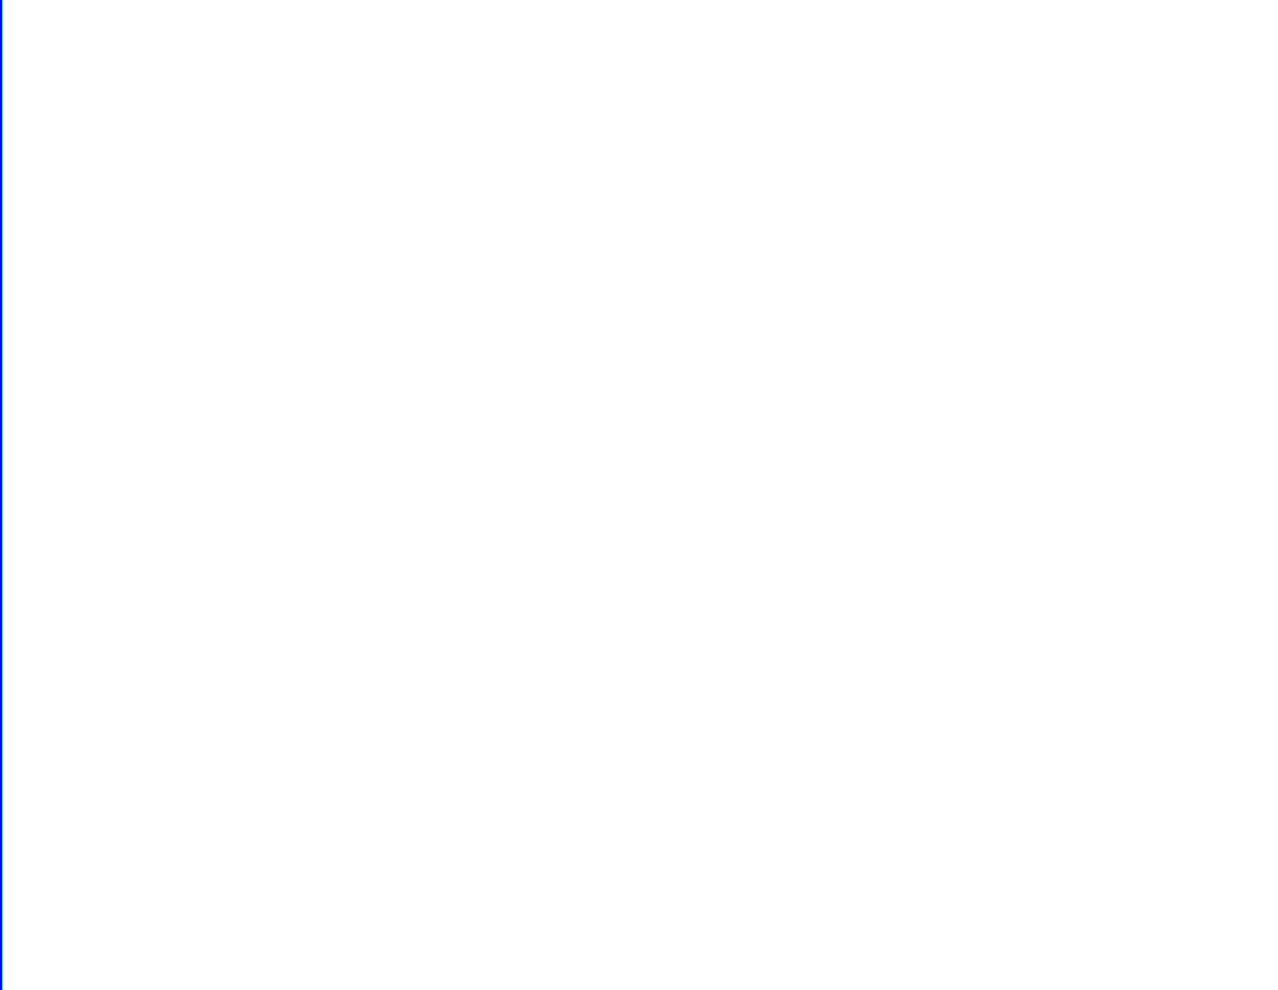
\includegraphics[width=\textwidth]{blank} % FIXME: insert the correct figure
                \caption{\dots}
                \label{fig:blank} % FIXME: insert the correct label
            \end{figure}

    \section{Progettazione} \label{sec:progettazione}

        \subsection{Use Case Diagram} \label{subsec:use-case-diagram}

            Come precedentemente descritto, il sistema è stato progettato per permettere agli utenti di creare eventi, partecipare a quelli creati da altri utenti e gestire il proprio profilo. \\
            La Figura~\ref{fig:use-case-diagram} mostra il diagramma dei casi d'uso del sistema, comprendendo sia gli use case degli utenti che degli amministratori.

            \begin{figure}[H]
                \centering
                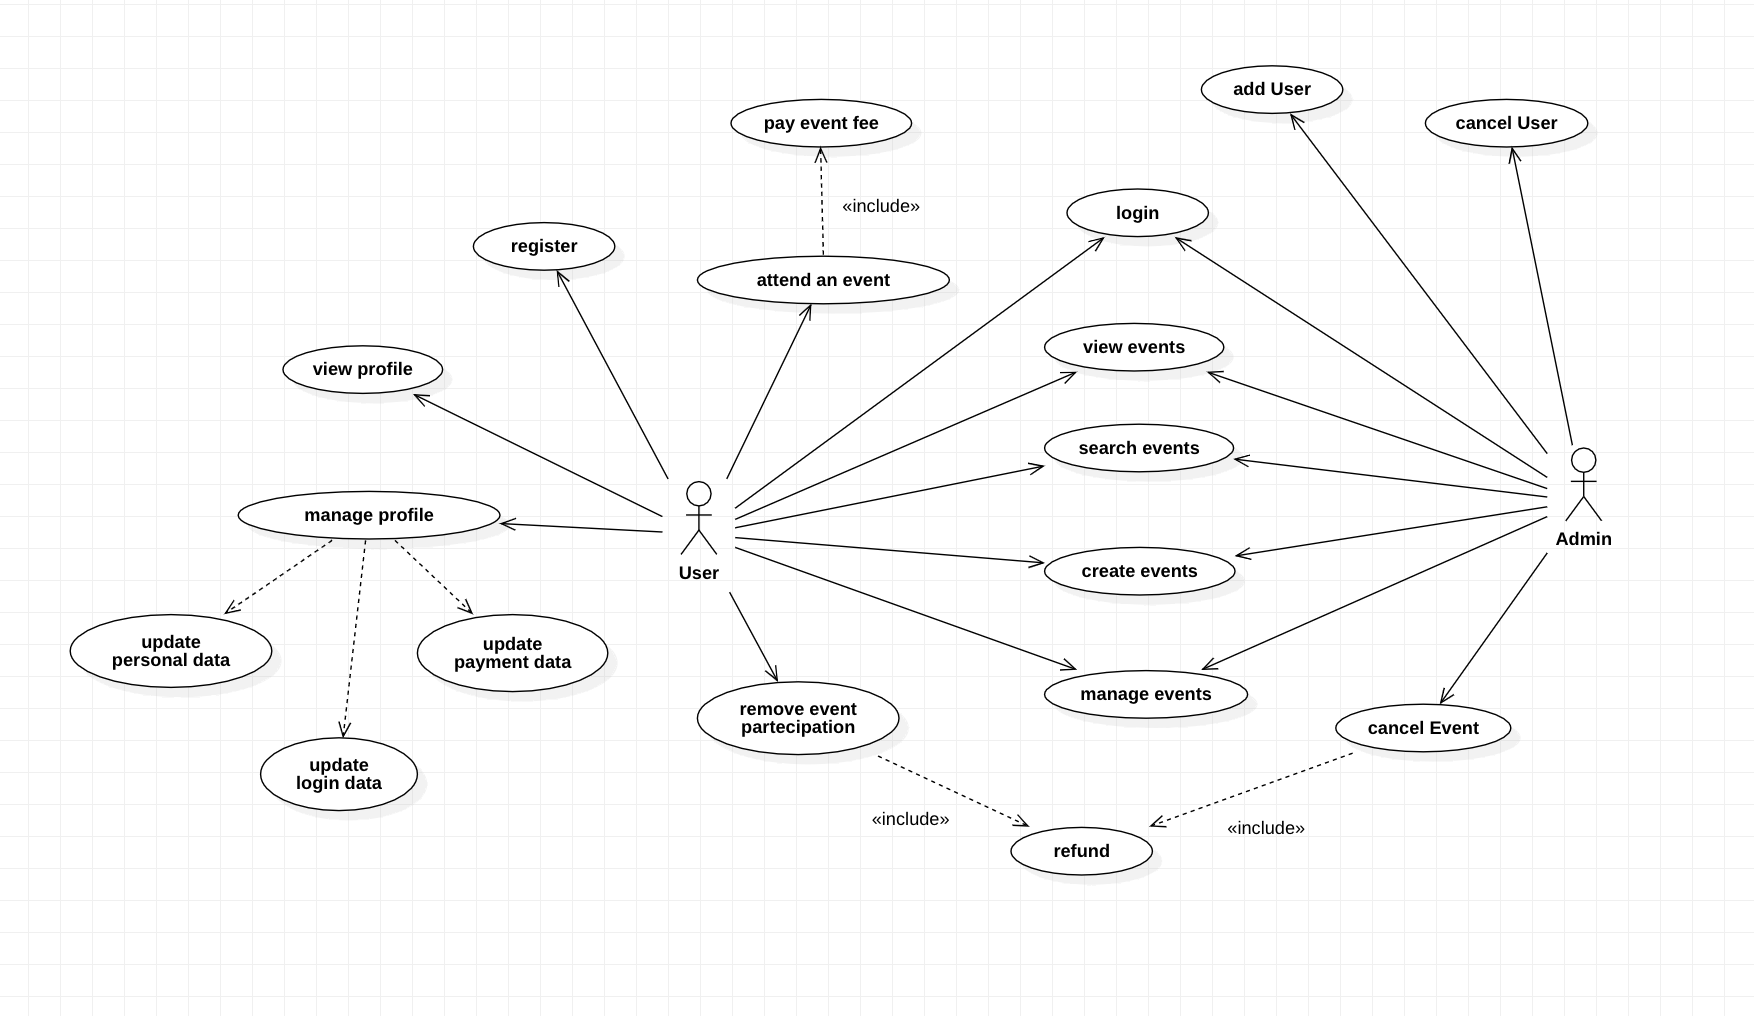
\includegraphics[width=\textwidth]{use_case_diagram/use_case_diagram}
                \caption{Use Case Diagram}
                \label{fig:use-case-diagram}
            \end{figure}

        \subsection{Use Case Template} \label{subsec:use-case-template}

            text

        \subsection{Mockups} \label{subsec:mockups}

            % TODO: rewrite (copied)
            Riporto di seguito alcuni possibili Mock-ups relativi alle interfacce grafiche di questo applicativo per l’interazione con gli attori esterni.


            \begin{figure}[H]
                \centering
                \setlength{\fboxsep}{10pt} % Adjust to your preference
                \tcbox[colframe=white,colback=darkgray,boxsep=2mm,arc=2mm]{ % Change 'darkgray' to your preferred color, adjust 'arc' for roundness
                    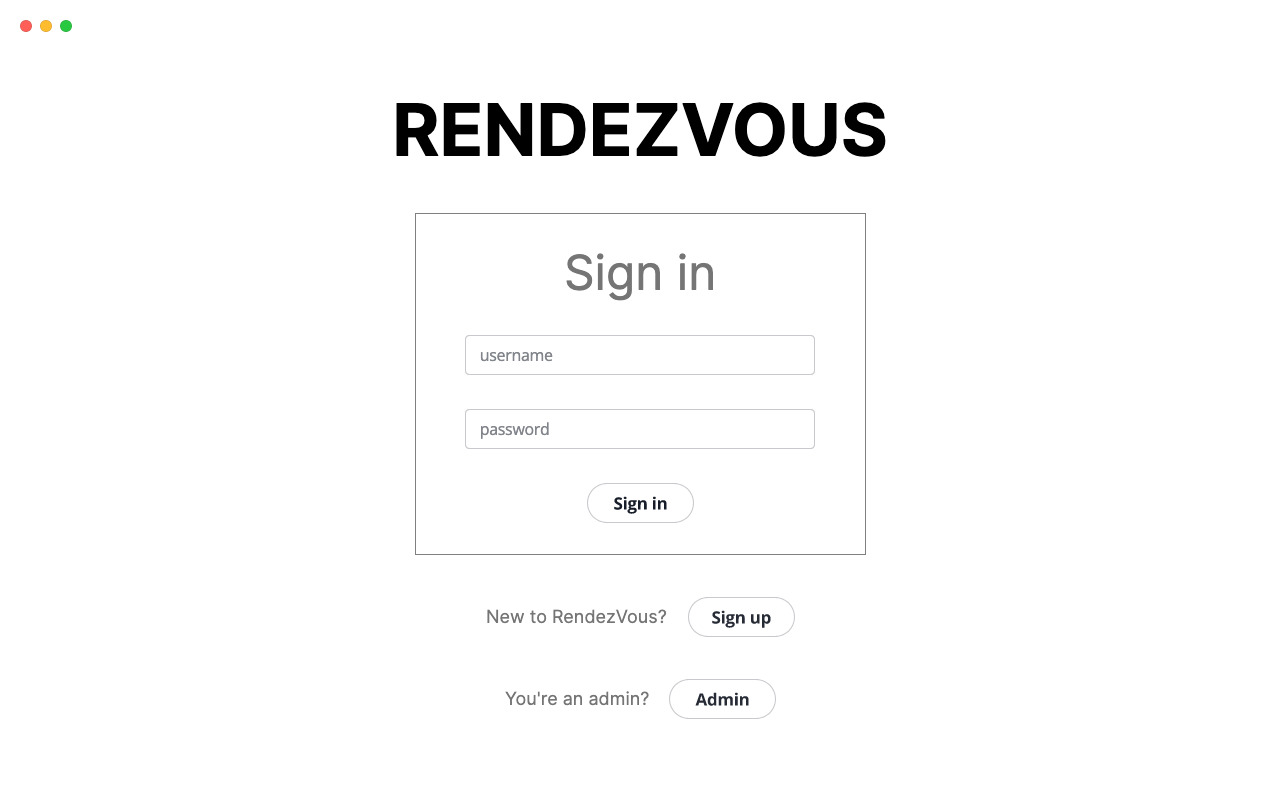
\includegraphics[width=\textwidth]{1/MK#1.1 - Sign in} % Adjust the width to your preference
                }
                \caption{Prototipo della pagina di Sign in}
                \label{fig:mockup-1.1}
            \end{figure}

            \setlength{\fboxsep}{10pt}
            \begin{figure}[H]
                \centering
                \setlength{\fboxsep}{10pt} % Adjust to your preference
                \tcbox[colframe=white,colback=darkgray,boxsep=2mm,arc=2mm]{ % Change 'darkgray' to your preferred color, adjust 'arc' for roundness
                    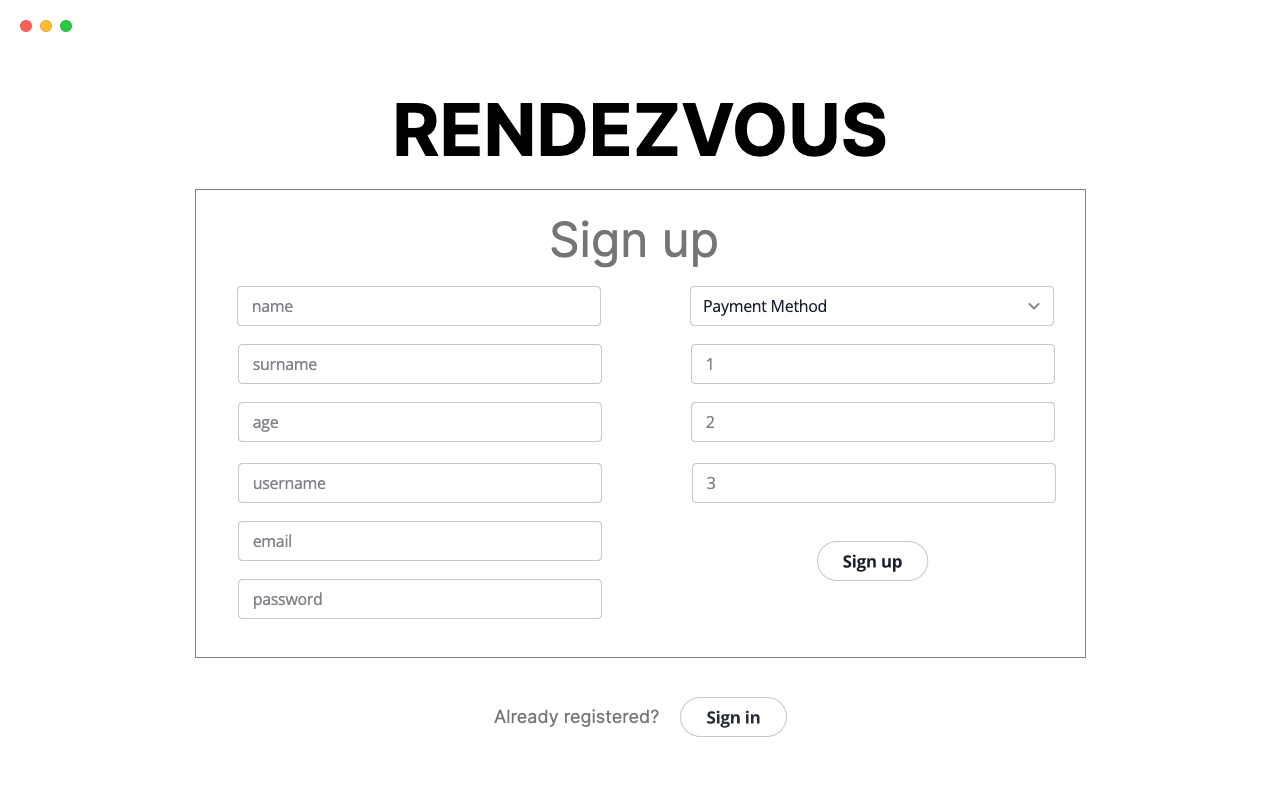
\includegraphics[width=\textwidth]{1/MK#1.2 - Sign up} % Adjust the width to your preference
                }
                \caption{Prototipo della pagina di Sign up}
                \label{fig:mockup-1.2}
            \end{figure}

            \setlength{\fboxsep}{10pt}
            \begin{figure}[H]
                \centering
                \setlength{\fboxsep}{10pt} % Adjust to your preference
                \tcbox[colframe=white,colback=darkgray,boxsep=2mm,arc=2mm]{ % Change 'darkgray' to your preferred color, adjust 'arc' for roundness
                    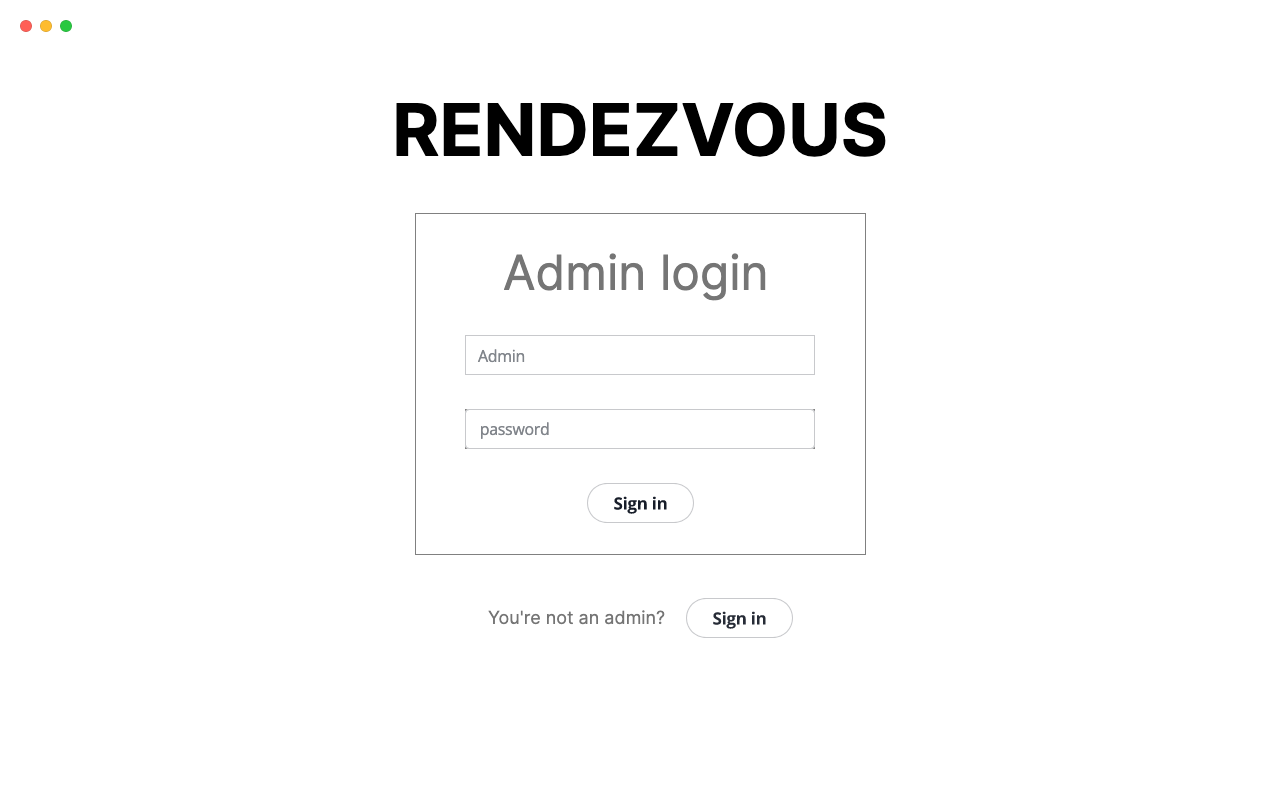
\includegraphics[width=\textwidth]{1/MK#1.3 - Admin login} % Adjust the width to your preference
                }
                \caption{Prototipo della pagina dell' Admin login}
                \label{fig:mockup-1.3}
            \end{figure}


    \subsection{Class Diagram} \label{subsec:class-diagram}

            text

            % TODO: think if it's bettere to keep the class diagrams separated or not

            \begin{figure}[H]
                \centering
                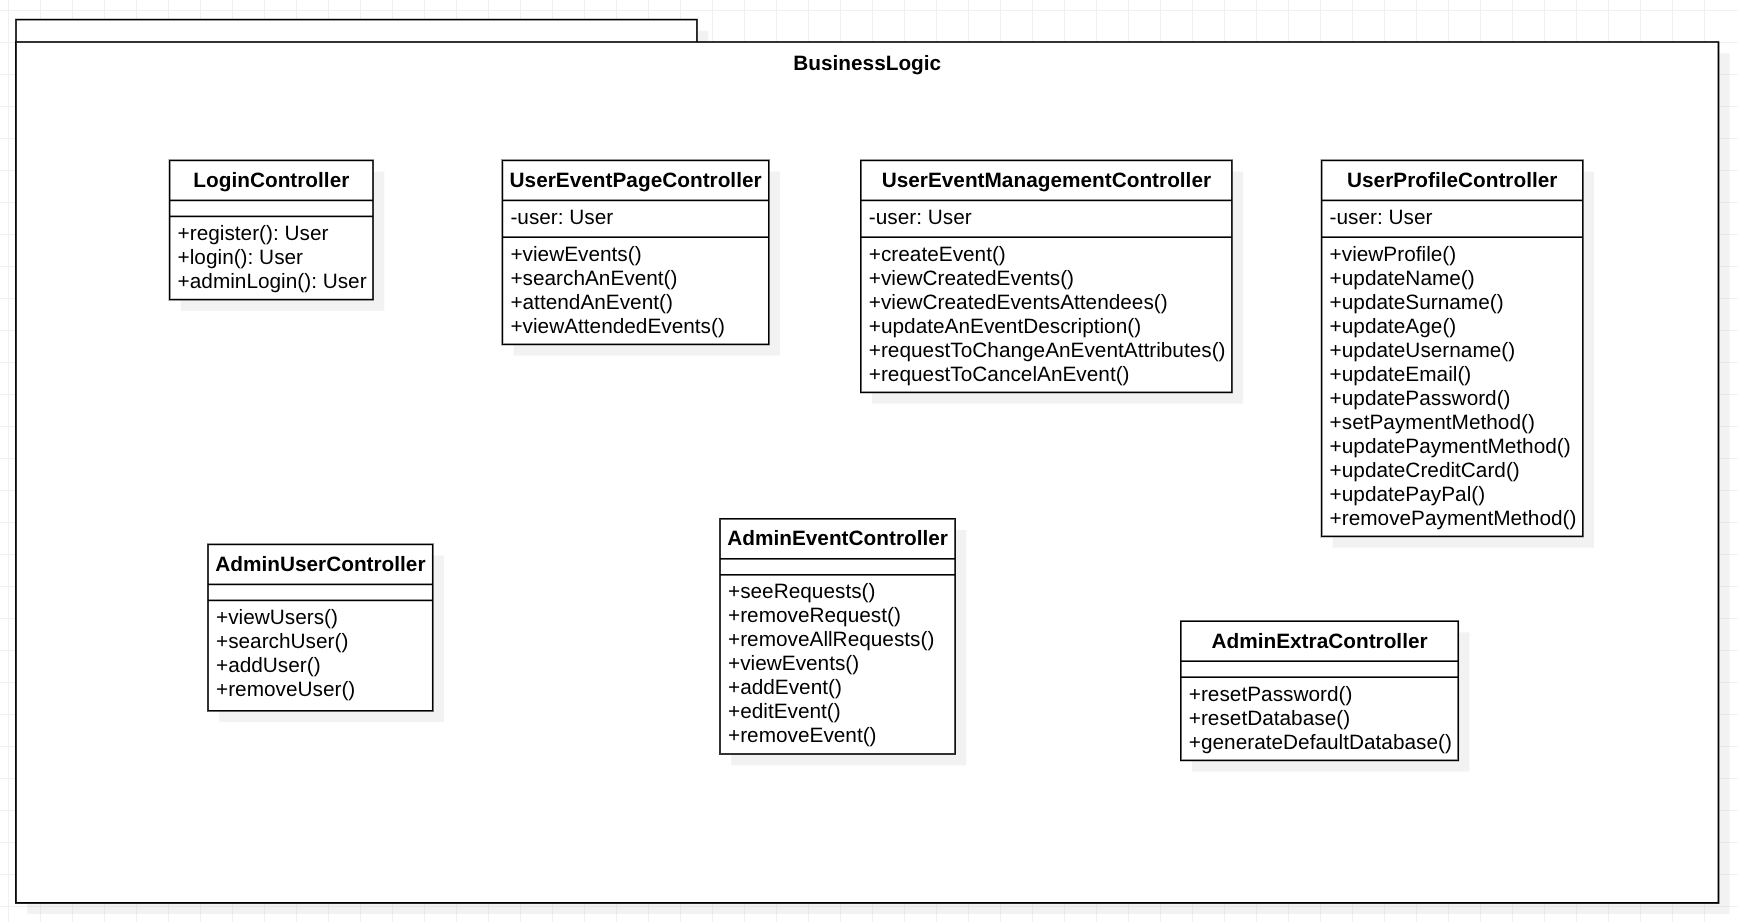
\includegraphics[width=\textwidth]{class_diagram/business_logic_tmp}
                \caption{Business Logic Class Diagram}
                \label{fig:business-logic-class-diagram}
            \end{figure}

            \begin{figure}[H]
                \centering
                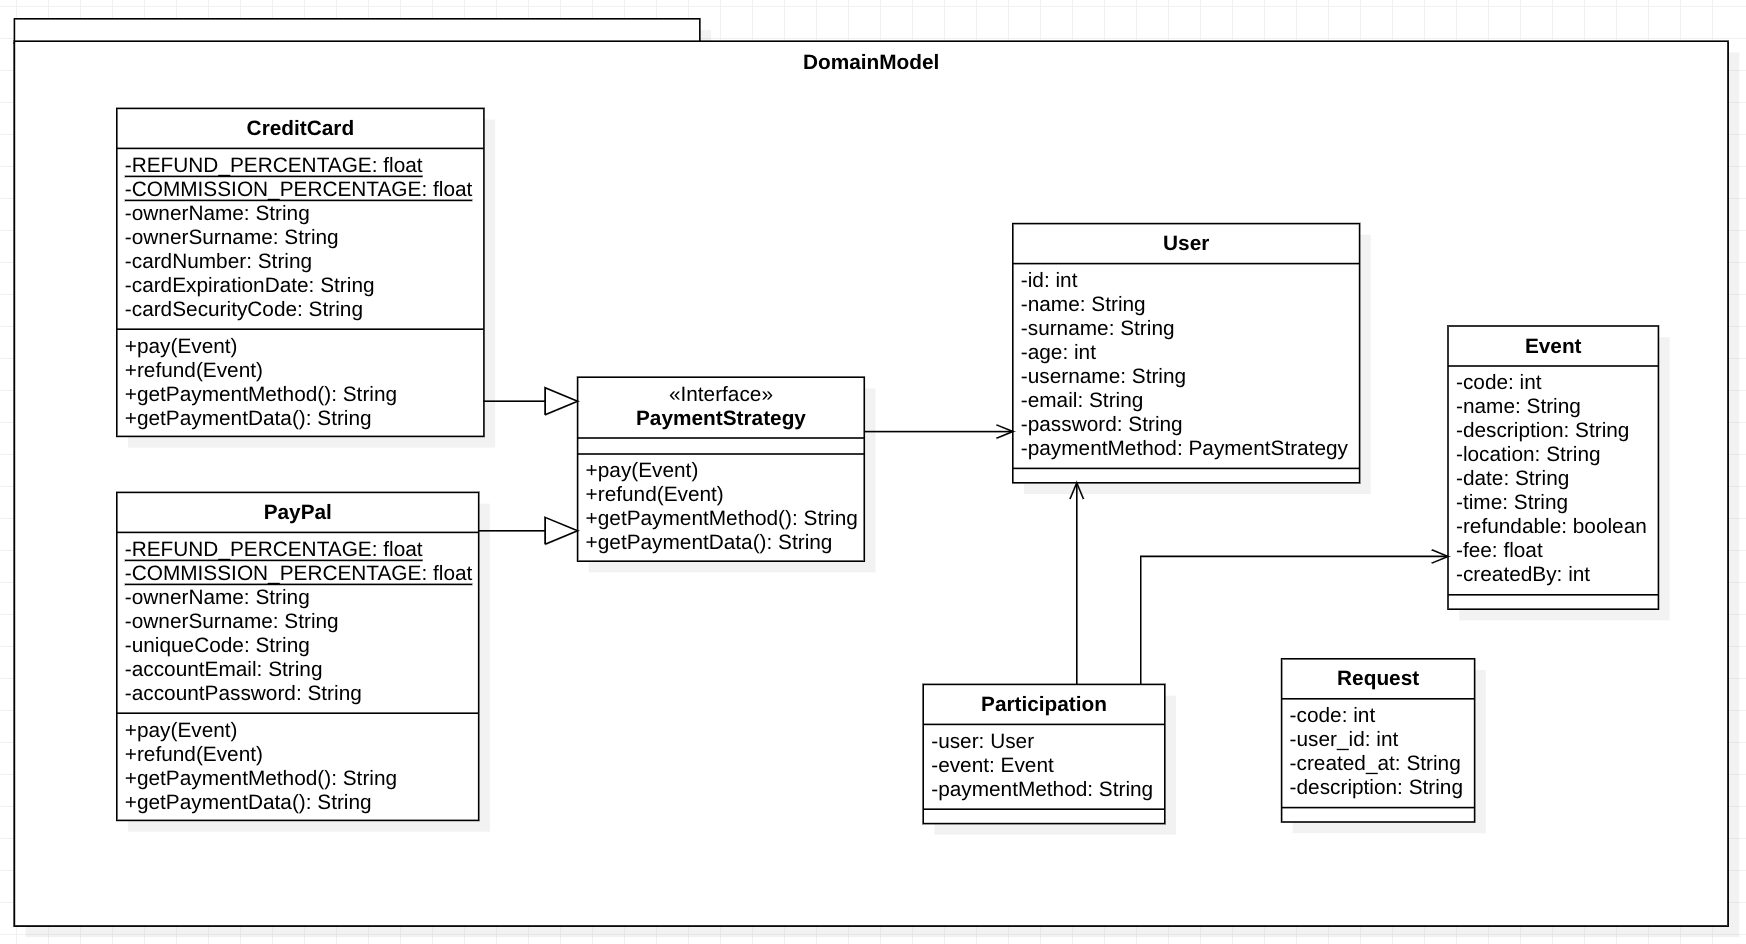
\includegraphics[width=\textwidth]{class_diagram/domain_model_tmp}
                \caption{Domain Model Class Diagram}
                \label{fig:domain-model-class-diagram}
            \end{figure}

            \begin{figure}[H]
                \centering
                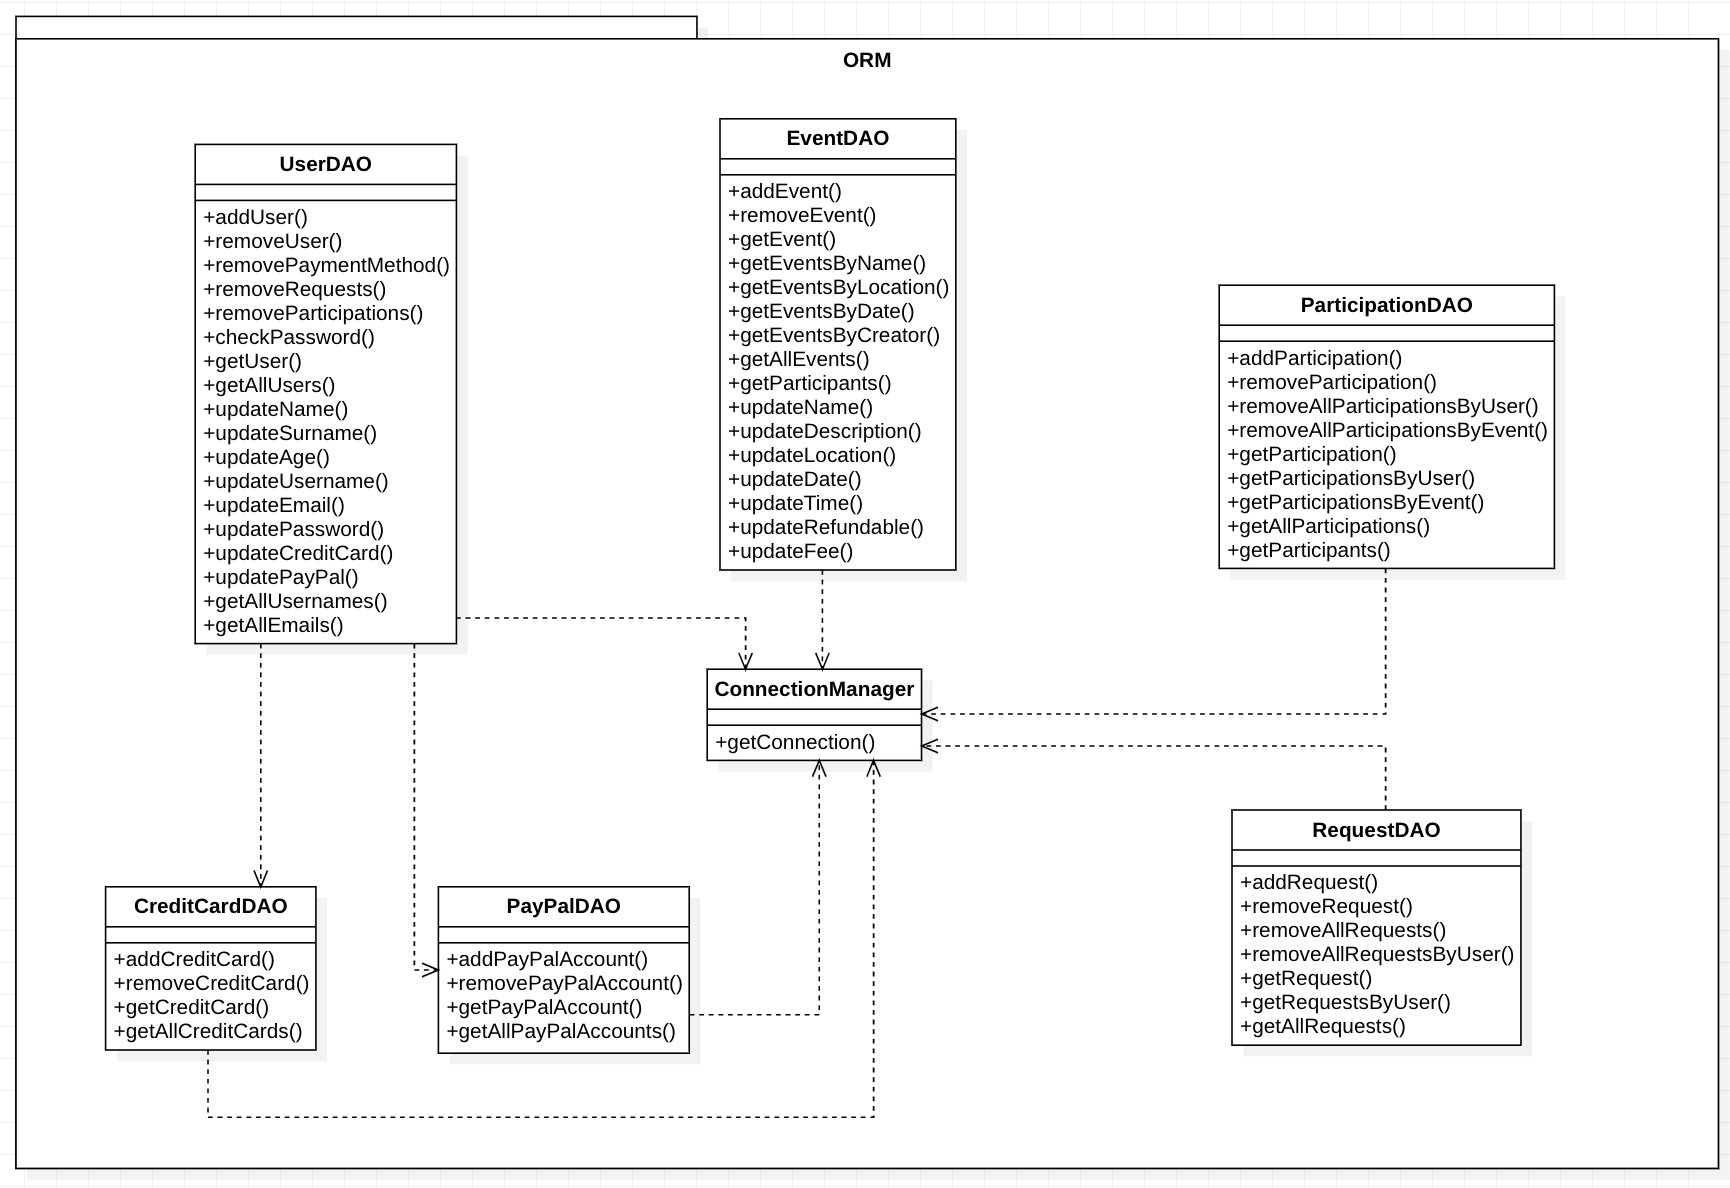
\includegraphics[width=\textwidth]{class_diagram/orm_tmp}
                \caption{ORM Class Diagram}
                \label{fig:orm-class-diagram}
            \end{figure}

            text

        \subsection{ER Diagram} \label{subsec:er-diagram}

            text

            \begin{figure}[H]
                \centering
                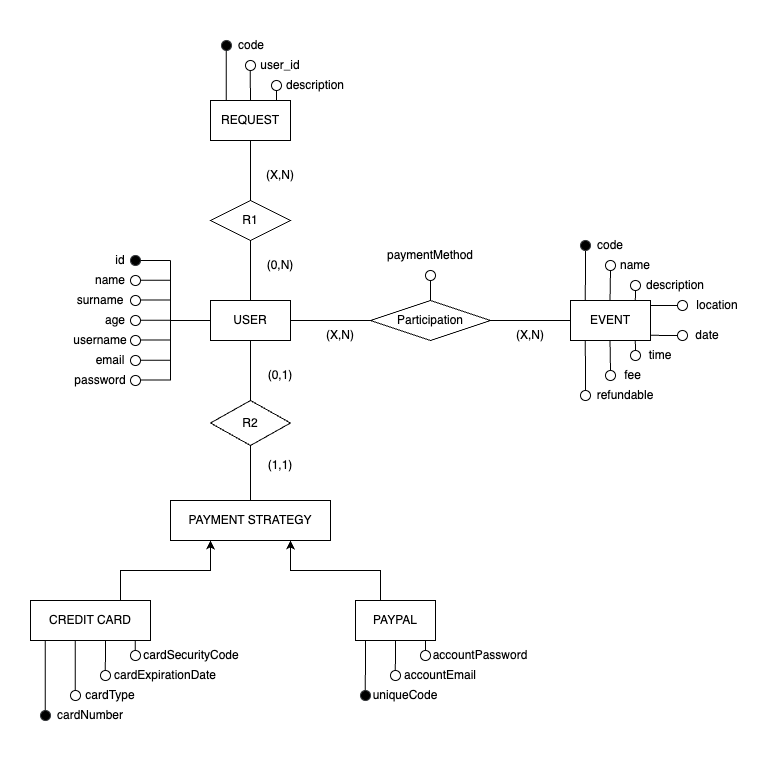
\includegraphics[width=\textwidth]{er_diagram/er_diagram}
                \caption{ER Diagram}
                \label{fig:er-diagram}
            \end{figure}

            \begin{figure}[H]
                \centering
                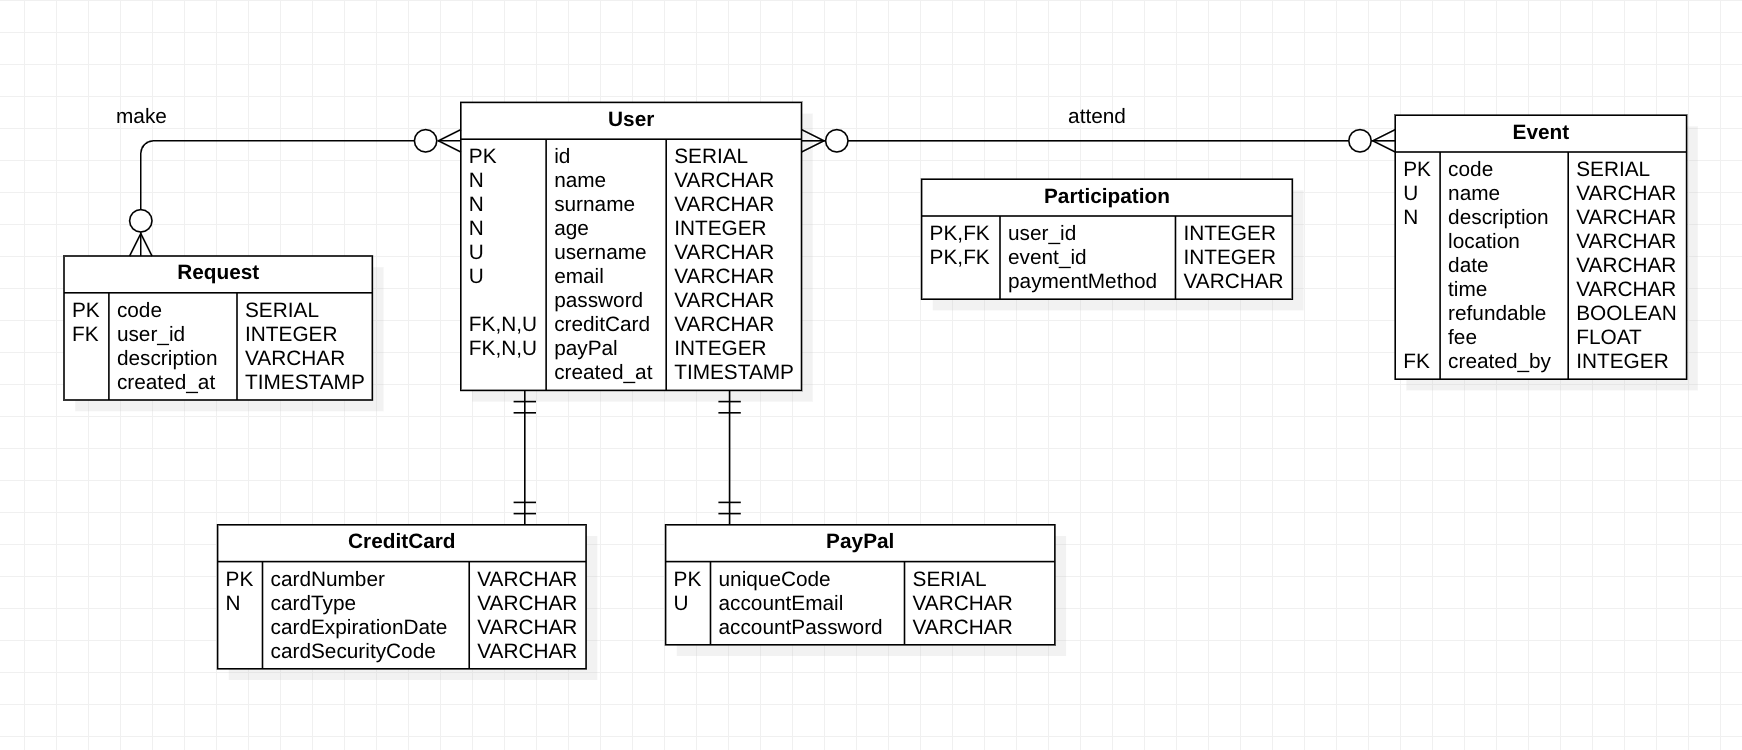
\includegraphics[width=\textwidth]{er_diagram/er_diagram_1}
                \caption{ER Diagram 1}
                \label{fig:er-diagram-1}
            \end{figure}

            \begin{figure}[H]
                \centering
                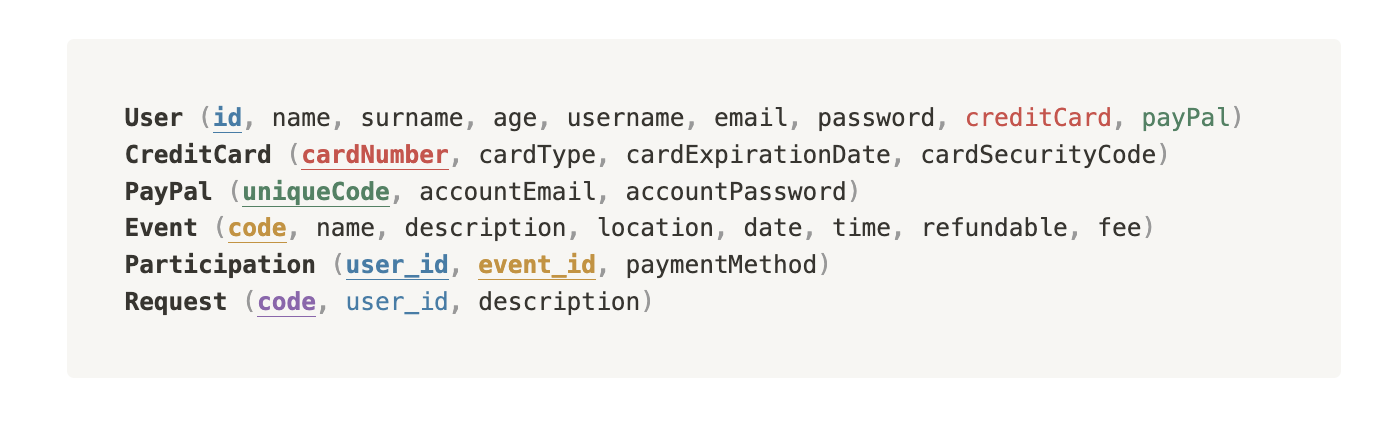
\includegraphics[width=\textwidth]{er_diagram/relational_model_1}
                \caption{Relational Model}
                \label{fig:relational-model}
            \end{figure}

            text

        \subsection{Navigation Diagram} \label{subsec:navigation-diagram}

            text

            \begin{figure}[H]
                \centering
                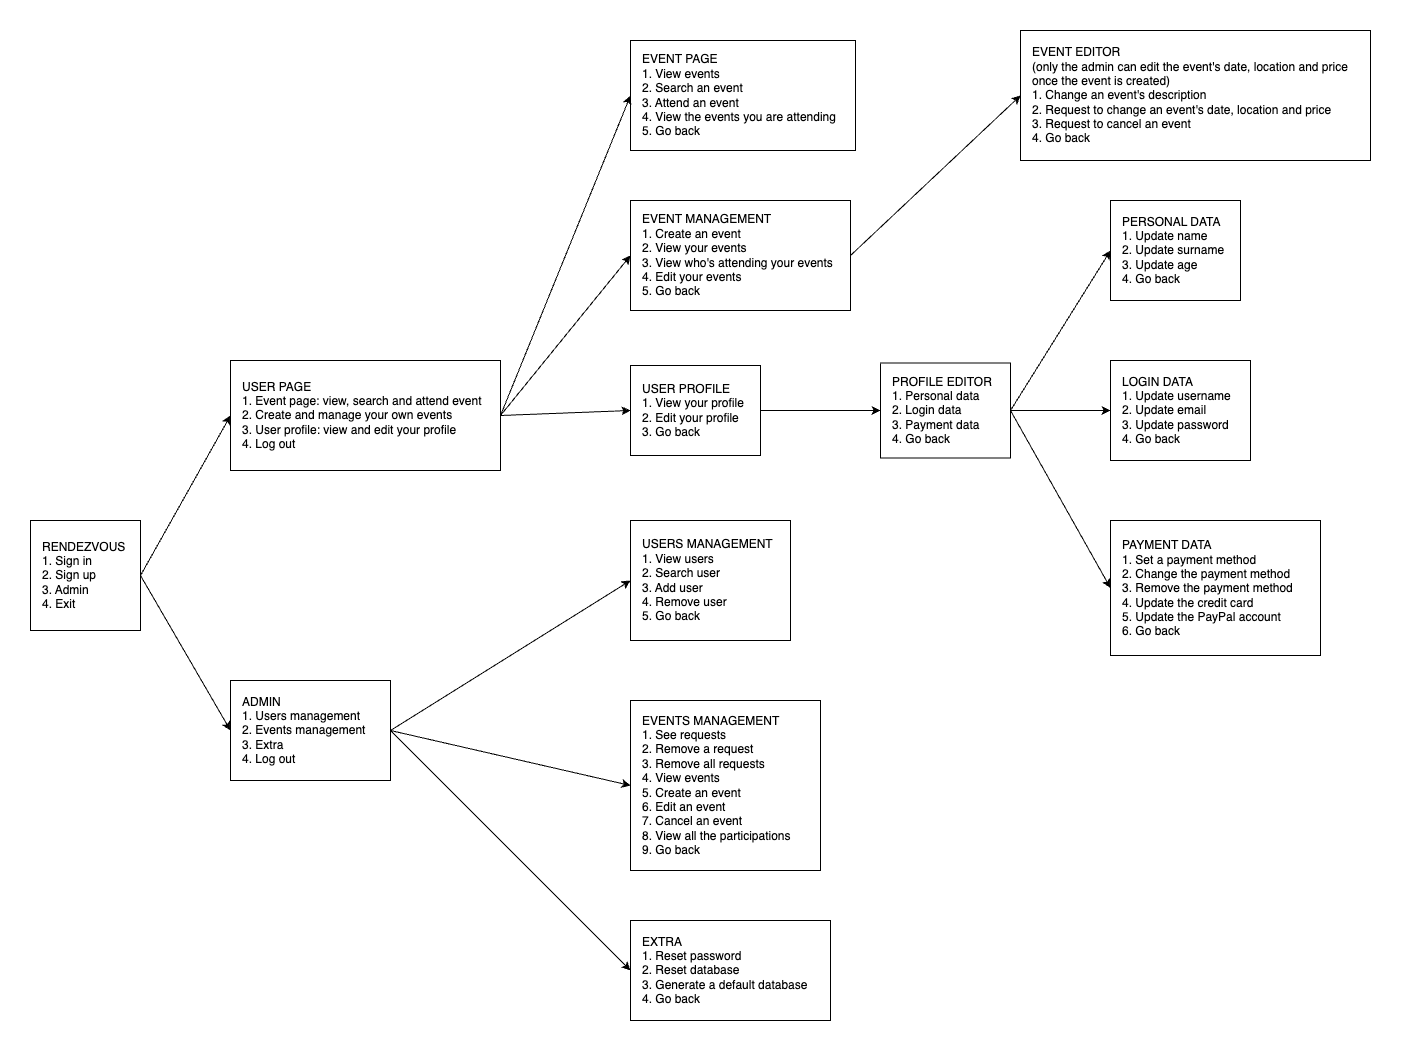
\includegraphics[width=\textwidth]{navigation_diagram/navigation_diagram}
                \caption{Navigation Diagram}
                \label{fig:navigation-diagram}
            \end{figure}

            text

        \subsection{Struttura delle directory} \label{subsec:struttura-delle-directory}

            text

            \begin{figure}[H]
                \centering
                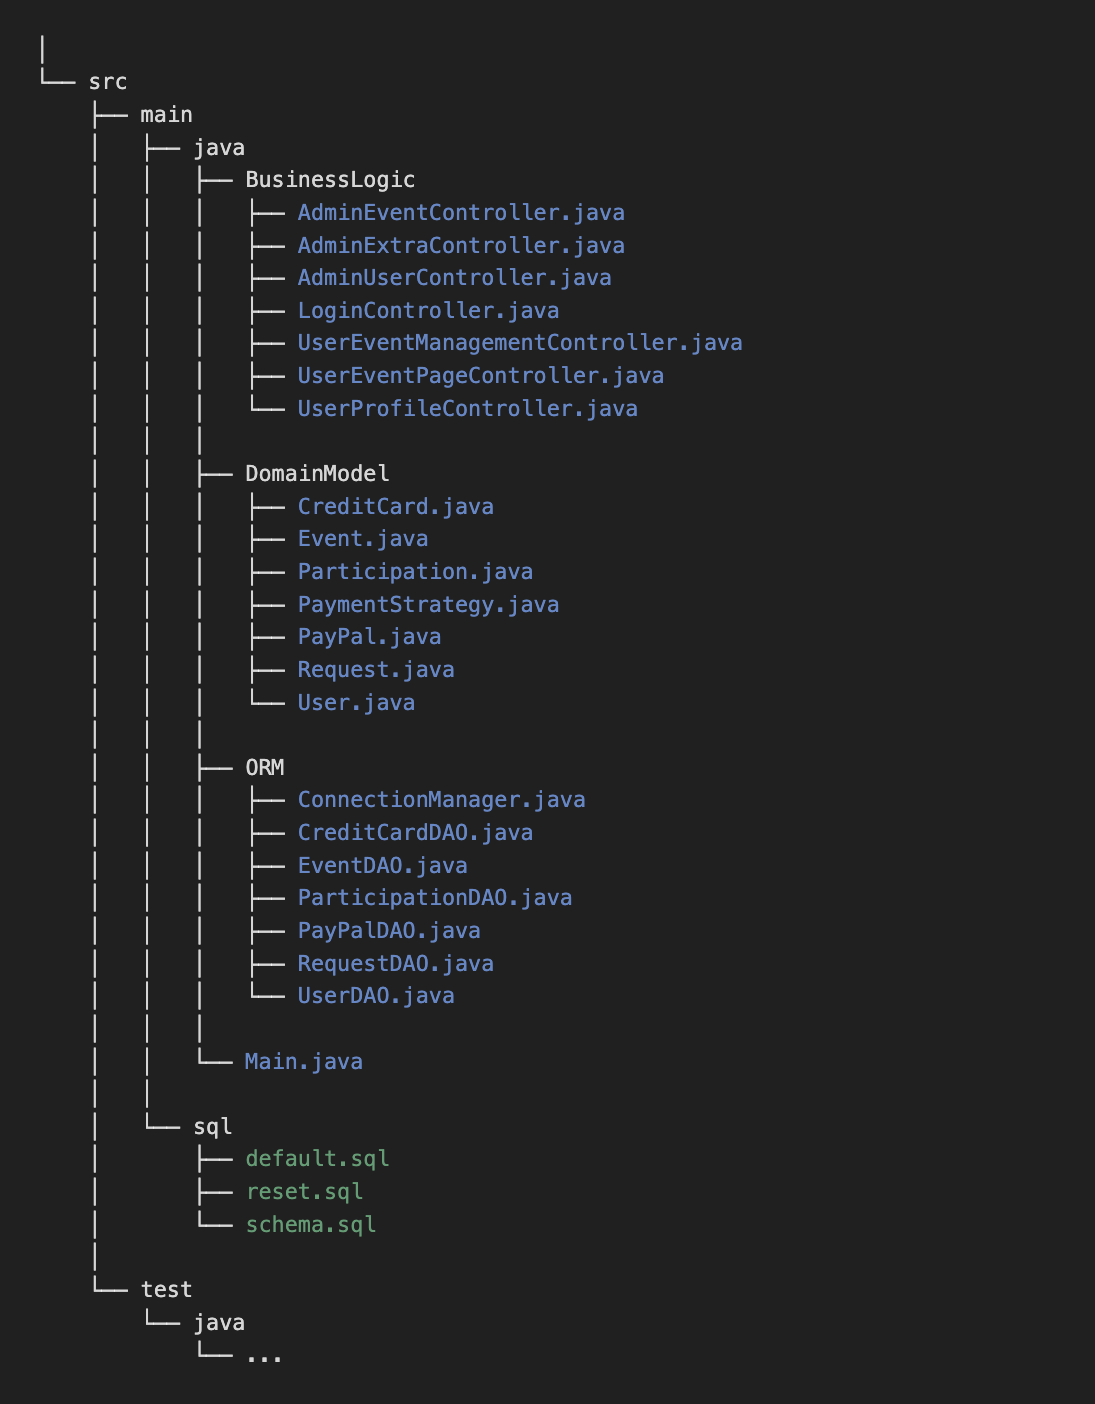
\includegraphics[width=\textwidth]{directory_structure_tmp}
                \caption{Struttura delle directory}
                \label{fig:directory-structure}
            \end{figure}

            text

    \section{Implementazione} \label{sec:implementazione}

        \subsection{Domain Model} \label{subsec:domain-model}

            text

            \subsubsection{User} \label{subsubsec:user}

                text

            \subsubsection{Event} \label{subsubsec:event}

                text

            \subsubsection{Participation} \label{subsubsec:participation}

                text

            \subsubsection{Request} \label{subsubsec:request}

                text

            \subsubsection{PaymentStrategy} \label{subsubsec:pament-strategy}

                text

            \subsubsection{CreditCard} \label{subsubsec:credit-card}

                text

            \subsubsection{PayPal} \label{subsubsec:paypal}

                text

        \subsection{Business Logic} \label{subsec:business-logic}

            text

            \subsubsection{LoginController} \label{subsubsec:login-controller}

                text

            \subsubsection{UserEventPageController} \label{subsubsec:user-event-page-controller}

                text

            \subsubsection{UserEventManagementController} \label{subsubsec:user-event-management-controller}

                text

            \subsubsection{UserProfileController} \label{subsubsec:user-profile-controller}

                text

            \subsubsection{AdminEventController} \label{subsubsec:admin-event-controller}

                text

            \subsubsection{AdminUserController} \label{subsubsec:admin-user-controller}

                text

            \subsubsection{AdminExtraController} \label{subsubsec:admin-extra-controller}

                text

        \subsection{ORM} \label{subsec:orm}

            text

            \subsubsection{ConnectionManager} \label{subsubsec:connection-manager}

                text

            \subsubsection{UserDAO} \label{subsubsec:user-dao}

                text

            \subsubsection{EventDAO} \label{subsubsec:event-dao}

                text

            \subsubsection{ParticipationDAO} \label{subsubsec:participation-dao}

                text

            \subsubsection{RequestDAO} \label{subsubsec:request-dao}

                text

            \subsubsection{CreditCardDAO} \label{subsubsec:credit-card-dao}

                text

            \subsubsection{PayPalDAO} \label{subsubsec:paypal-dao}

                text

        \subsection{Database} \label{subsec:database}

            text

    \section{Testing} \label{sec:testing}

        text

        \subsection{Business Logic Testing} \label{subsec:business-logic-testing}

            text

        \subsection{Domain Model Testing} \label{subsec:domain-model-testing}

            text

        \subsection{ORM Testing} \label{subsec:orm-testing}

            text

\end{document}